%%%%%%%%%%%%%%%%%%%%%%%%%%%%%%%%%%%%%%%%%%%%%%%%%%%%%%%%%%%%%%%%%%
%%%%%%%% ICML 2015 EXAMPLE LATEX SUBMISSION FILE %%%%%%%%%%%%%%%%%
%%%%%%%%%%%%%%%%%%%%%%%%%%%%%%%%%%%%%%%%%%%%%%%%%%%%%%%%%%%%%%%%%%

% Use the following line _only_ if you're still using LaTeX 2.09.
%\documentstyle[icml2015,epsf,natbib]{article}
% If you rely on Latex2e packages, like most moden people use this:
\documentclass[10pt]{article}

% use Times
\usepackage{times}
% For figures
\usepackage{graphicx} % more modern
%\usepackage{epsfig} % less modern
\usepackage{float}

% For citations
\usepackage{natbib}

% For algorithms
\usepackage{algorithm}
\usepackage{algorithmic}
\usepackage{bm}
\usepackage{amssymb,amsmath}


% As of 2011, we use the hyperref package to produce hyperlinks in the
% resulting PDF.  If this breaks your system, please commend out the
% following usepackage line and replace \usepackage{icml2015} with
% \usepackage[nohyperref]{icml2015} above.
\usepackage{hyperref}

% Packages hyperref and algorithmic misbehave sometimes.  We can fix
% this with the following command.
\newcommand{\theHalgorithm}{\arabic{algorithm}}

% Employ the following version of the ``usepackage'' statement for
% submitting the draft version of the paper for review.  This will set
% the note in the first column to ``Under review.  Do not distribute.''
\usepackage[accepted]{icml2015}
\usepackage{amsmath}
\usepackage{amsmath}
\usepackage{amsfonts}
\usepackage{amssymb}

\usepackage{todonotes}

\usepackage{amsbsy}

% Employ this version of the ``usepackage'' statement after the paper has
% been accepted, when creating the final version.  This will set the
% note in the first column to ``Proceedings of the...''
%\usepackage[accepted]{icml2015}


% The \icmltitle you define below is probably too long as a header.
% Therefore, a short form for the running title is supplied here:

% Saving space by deleting running title (does this actually save space?)
%\icmltitlerunning{Submission and Formatting Instructions for ICML 2015}

\begin{document} 

\twocolumn[

% Saving space by deleting title
%\icmltitle{Submission and Formatting Instructions for \\ 
%           International Conference on Machine Learning (ICML 2015)}

% It is OKAY to include author information, even for blind
% submissions: the style file will automatically remove it for you
% unless you've provided the [accepted] option to the icml2015
% package.


% You may provide any keywords that you 
% find helpful for describing your paper; these are used to populate 
% the "keywords" metadata in the PDF but will not be shown in the document
\icmlkeywords{6.867, machine learning}

\vskip 0.3in
]

% Saving space by deleting abstract
%\begin{abstract} 
%The purpose of this document is to provide both the basic paper template and
%submission guidelines.
%\end{abstract} 

\section{Logistic Regression}



We used our gradient descent code from Homework 1 to solve this problem. In particular we supplied the optimizer with analytic gradients. If we define $\tilde{x}$ to be $[1,x]^T$ then the gradient of the regularized NLL objective can be written as
%
%
\begin{equation}
\frac{\partial E_{LR}(w)}{\partial w} = \sum_i -y^{(i)} \tilde{x}^{(i)} \frac{\exp(-y^{(i)}(\tilde{x}^{(i)}w + w_0))}{1 + \exp(-y^{(i)}(\tilde{x}^{(i)}w + w_0))}
\end{equation}
%
%
As was shown in lecture, the objective function for logistic regression is convex. Thus gradient descent should, with the appropriate step size and convergence threshold, converge to the global minimum. For almost all the subsequent optimizations we used a step size of $\eta = 1e-4$ and an initial guess of $w_{initial} = [0,0,0]$. A few optimizations (in particular those for very large $\lambda$) required a smaller step size, approximately $\eta = 1e-6$.

\subsection*{Results for $\lambda = 0$}

First we present the results for $\lambda = 0$ in Table \ref{lam_0}
\begin{table}[H]
\begin{tabular}{|c|c|}
\hline
\textbf{Dataset} & \textbf{Misslassification rate} \\ \hline
stdev1 train & $0$\\ \hline
stdev1 val & $0$\\ \hline
stdev2 train & $0.0925$\\ \hline
stdev2 val & $0.08$\\ \hline
stdev4 train & $0.26$\\ \hline
stdev4 val & $0.25$\\ \hline
nonsep train & $0.485$\\ \hline
nonsep val & $0.5025$\\ \hline
\end{tabular}

\caption{Results on different dataset for $\lambda = 0$}
\label{lam_0}
\end{table}


 Define $\tilde{w} = [w_0,w]$ to be the full weight vector. For the datasets stdev1, stdev2, stdev4 the gradient descent method converges to solution. The stdev1 dataset is linearly separable. This presents a problem for the optimizer since given a weight $\tilde{w}$ that separates the data, we can arbitrarily increase the value of the likelihood by considering new weights $c \tilde{w}$ where $c > 1$ is a constant. In practice our gradient descent method always terminates because either the termination criterion is reached (e.g. difference in function values on successive steps is smaller than a threshold) or we reach the maximum number of function calls. As an illustration if we run the optimizer with termination criterion $\epsilon = 1e-4$ we get $||\tilde{w}|| = 7.9$. If we increase the tolerance to $\epsilon = 1e-10$ then the norm of the solution weights increases to $||\tilde{w}|| = 14.7$. This illustrates the weights ``running off to infinty''. Since the training data is linearly separable the classification error rate is zero. Also as can be seen from Figure \ref{stdev1_val_lam_0} the classification error rate on the validation data is also zero.

% \begin{figure}
%  \centering
%  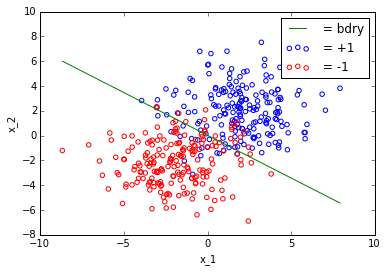
\includegraphics[scale=0.5]{stdev1_train_lam_0.png}
%  \label{stdev1_train_lam_0}
%  \caption{$\lambda = 0$, stdev1 train dataset}
%  \label{stdev1_train_lam_0}
%  \end{figure}

\begin{figure}
 \centering
 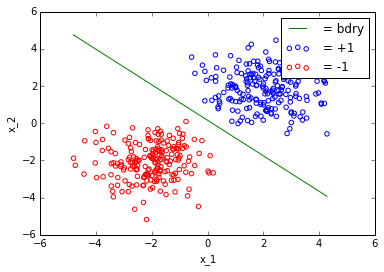
\includegraphics[scale=0.5]{stdev1_val_lam_0.png}
 
 \caption{$\lambda = 0$, stdev1 validation dataset}
 \label{stdev1_val_lam_0}
 \end{figure}
 % \quad
 % \subfloat[Run 2]{%
 % 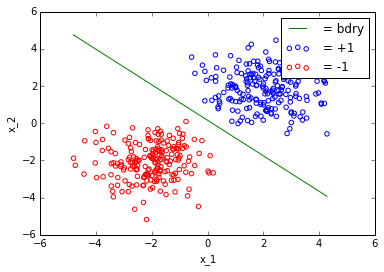
\includegraphics[scale=0.5]{stdev1_val_lam_0.png}
 % \label{stdev1_val_lam_0}
 % }
 % \caption{Results of logistic regression with $\lambda = 0$ for the training and validation sets.}
 % \end{figure} 

The other datasets (other than stdev1) are not linearly separable. Hence we don't have the ``weights running off to infinity'' problem that we had with stdev1. Since the stdev of the points in these datasets is larger (making them non-separable) we also expect the classfication error rate to be larger as well. The results for the stdev4 dataset are shown in Figures \ref{stdev4_train_lam_0} and \ref{stdev4_val_lam_0}. The classifier still exihibits relatively good performance in separating the data. Even though the data is noisy, the decision boundary is very similar to the one in the less noisy case, the stdev1 data.
\begin{figure}
 \centering
 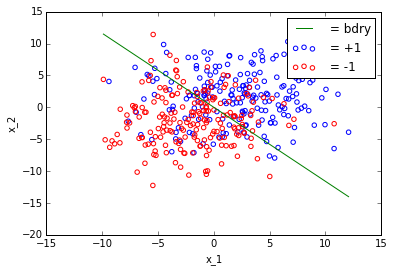
\includegraphics[scale=0.5]{stdev4_train_lam_0.png}
 
 \caption{Results for $\lambda = 0$, stdev4 train dataset}
 \label{stdev4_train_lam_0}
 \end{figure}

\begin{figure}
 \centering
 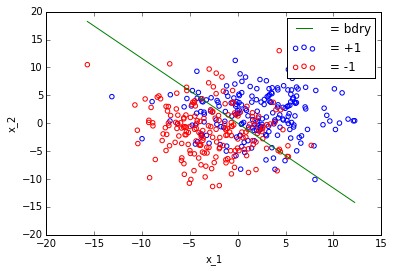
\includegraphics[scale=0.5]{stdev4_val_lam_0.png}
 
 \caption{$\lambda = 0$, stdev4 validation dataset}
 \label{stdev4_val_lam_0}
 \end{figure}
 %
 %
 In contrast the performance on the nonseparable dataset is quite poor. This makes sense since the data is not linearly separable.
\begin{figure}[H]
 \centering
 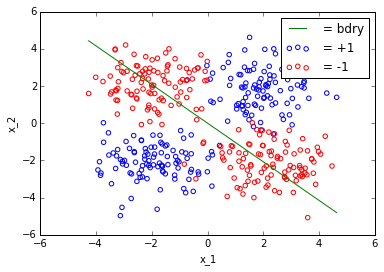
\includegraphics[scale=0.5]{nonsep_train_lam_0.png}
 
 \caption{$\lambda = 0$, nonsep train dataset}
 \label{nonsep_train_lam_0}
 \end{figure}

 Interestingly, even with the regularizer $\lambda$ set to $0$ the performance across the training and validation sets for a given dataset (e.g. stdev2) are comparable. This can be seen by the similar missclassification rates across corresponding training and validation sets in Table \ref{lam_0}. This means that our logistic regression classifier is generalizing fairly well.


\subsection*{Results for $\lambda > 0$}
Now we analyze the results for different values of the regularizer $\lambda$. Figures \ref{nonsep_train_lam_10}, \ref{nonsep_train_lam_100}, \ref{nonsep_train_lam_1000} shows the result of running logistic regression on the nonsep dataset for different values of $\lambda$. The thing to note is that for different values of $\lambda$ the actual decision boundary, plotted in green, looks very similar. In fact what seems to be happening is that as $\lambda$ increases the optimal weight $w(\lambda)$ are just scaled down to zero. In fact if we define $\overline{w}(\lambda) = \frac{w(\lambda)}{||w(\lambda)||}$ then $\overline{w}(\lambda)$ is very similar across different values of $\lambda$. Thus the regularizer $\lambda$ is forcing the weights toward zero, i.e. $||w(\lambda)||$ is decreasing in $\lambda$, but the scaled weights $\overline{w}(\lambda)$ are staying essentially the same. This explains why the decision boundaries look the same across the three plots in Figure \ref{nonsep_train_lam_10}, \ref{nonsep_train_lam_100} and \ref{nonsep_train_lam_1000} since $w_0 + w_1 x_1 + w_2 x_2 = 0$ and $c w_0 + c w_1 x_1 + c w_2 x_2 = 0$ (where $c > 0$ is a constant) define the same hyperplane. Thus in this case the regularizer $\lambda$ just serves to drive the weights toward zero, but does so in a way that doesn't significantly affect the classification boundary. Table \ref{w_lam_norm} shows how $||\tilde{w}(\lambda)|| \to 0$ as we increase $\lambda$.

The results on the other datasets (stdev1, stdev2, stdev4) are very similar. We see that as $\lamba$ increases the decision boundary stays almost the same, but the norm of the weights $||\tilde{w}(\lambda)||$ tends to zero. 

\begin{table}[H]
\begin{tabular}{|c|c|c|}
\hline
$\lambda$ & $||\tilde{w}(\lambda)||$ & CER on Validation Data\\ \hline
$0$ & $0.034$ & $0.5075$ \\ \hline
$10$ & $0.0329$ & $0.5075$ \\ \hline
$100$ & $0.0242$ & $0.505$\\ \hline
$1000$ & $0.00067$ & $0.505$ \\ \hline
\end{tabular}
%
%


\caption{Norm of $\tilde{w}(\lambda)$ for different values of $\lambda$ on nonsep train dataset.}
\label{w_lam_norm}
\end{table}

\begin{figure}
 \centering
 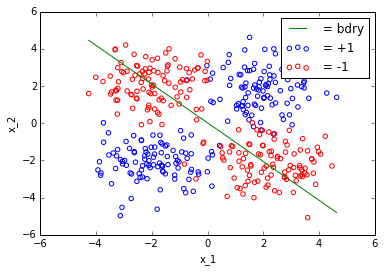
\includegraphics[scale=0.5]{nonsep_train_lam_10.png}
 \caption{$\lambda = 10$, nonsep train dataset}
  \label{nonsep_train_lam_10}
 \end{figure}
 \begin{figure}
 \centering
 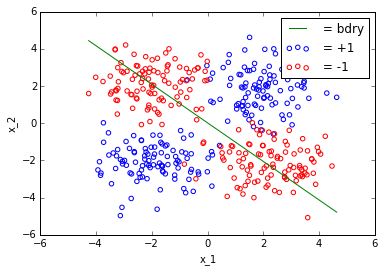
\includegraphics[scale=0.5]{nonsep_train_lam_100.png}
 \caption{$\lambda = 100$, nonsep train dataset}
 \label{nonsep_train_lam_100}
 \end{figure}
 \begin{figure}
 \centering
 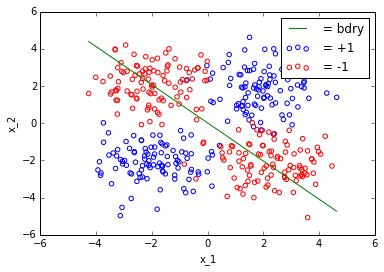
\includegraphics[scale=0.5]{nonsep_train_lam_1000.png}
 \caption{$\lambda = 1000$, nonsep train dataset}
 \label{nonsep_train_lam_1000}
 \end{figure}




\section{Support Vector Machine (SVM)}

%We implemented the dual form of Soft-SVMs.  Our implementation is general and capable of handling linear, Gaussian, or other user-specified kernels or Gram matrices, and allows the user to additionally specify $C$ (the variable that adjusts the relative penalty on the slack variables) and any special kernel-dependent variables (including the bandwidth for the Gaussian kernel).  

A description of the implementation is as follows.  Given a kernel function, $k(\cdot,\cdot)$, a set of N data points $\{x^{(i)}, y^{(i)}\}$ where each each $\mathbf{x} \in \mathbb{R}^d$ is paired with a a target label $t \in \{-1,1\}$, and $C$ as mentioned above, we can solve the dual form Soft-SVM optimization problem:
%
\begin{equation}
\begin{aligned}
& \underset{\alpha \in \mathbb{R}^N}{\text{maximize}} && \sum_{n=1}^N a_n - \frac{1}{2} \sum_{n=1}^N \sum_{m=1}^N a_na_mt_nt_mk(\mathbf{x}_n, \mathbf{x}_m)\\
& \text{subject to}
&& 0 \le a_n \le C \\
&&&\sum_{n=1}^N a_nt_n = 0
\end{aligned}
\end{equation}
%
The decision variables in the optimization are the elements $a_i, i =0,1,...,n$.  As the objective is quadratic and the constraints are linear inequalities and a linear equality, we solve the problem as a QP (Quadratic Program), using CVXOPT.  The QP interface to CVXOPT accepts problems in the form:
\begin{equation}
\begin{aligned}
& \text{minimize} && \frac{1}{2}a^TPa + q^Ta\\
& \text{subject to}
&& Ga \le h \\
&&& Aa = b
\end{aligned}
\end{equation}
A correct formulation of our Soft-SVM for the CVXOPT interface is accordingly: $P = \mathbf{t}\mathbf{t}^T K$ (where $K$ is the Gram matrix for the kernel), $q$ is a vector of length $N$ with each element $-1$, $G$ is a vertically stacked block matrix $[G_0; G_C]$ where $G_0$ and $G_C$ are both $N \times N$ diagonal matrices with, respectively, $-1$ and $1$ down the diagonals,  $H$ is a vector of length $2N$ where the first $N$ elements are zero and the last $N$ elements are each $C$, $A$ is $\mathbf{t}^T$, and $b = 0$.

For the example of 4 data points given, our $P$ matrix will be given by exactly:

\begin{equation}
\begin{aligned}
& t = \begin{bmatrix} 1 & 1 & -1 & -1 \end{bmatrix}^T \\
& K = \begin{bmatrix} 
5 & 6 & 0 & 4  \\
6 & 8 & 0 & 2  \\
0 & 0 & 0 & 0  \\
4 & 2 & 0 & 13  \\
\end{bmatrix} \\
& P =  \mathbf{t}\mathbf{t}^T K\\
\end{aligned}
\end{equation}
The Gram matrix $K$ is computed by pairwise dot product between points.  For the rest of the optimization matrices and vectors, $q$, $G$, and $h$ (note that $G,h,a,b$ correspond to the constraints) are simply constructed to be the right size, with $N=4$, as explained above, $A$ is $\mathbf{t}^T$, and $b$ still $0$.

%\begin{figure}
%\centering
%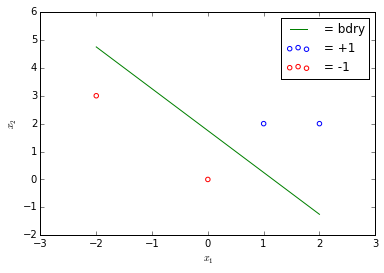
\includegraphics[scale=0.5]{svm_toy.png}
%\label{svm_toy}
%\caption{Soft-SVM solution for decision boundary of simple 2D dataset with $C=1$}
%\end{figure}

For the prediction function, we must first compute $b$ as follows:

\begin{equation}
\begin{aligned}
b = \frac{1}{N_\mathcal{M}} \sum_{n \in \mathcal{M}} \bigg(t_n  - \sum_{m \in \mathcal{S}} a_mt_mk(\mathbf{x}_n, \mathbf{x}_m) \bigg)
\end{aligned}
\end{equation}

where $\mathcal{S}$ denotes the set of indices of the support vectors, $\mathcal{M}$ denotes the set of indices of the strict support vectors (those that lie on the margin), and $N_{\mathcal{M}}$ is the number of strict support vectors.  The set $\mathcal{S} = \{n : a_n > 0\}$ and $\mathcal{M} =\{n : 0 < a_n < C\}$. With $b$, the prediction function is then simply: 
\begin{equation}
\begin{aligned}
y(\mathbf{x}) = \sum_{n=1}^N a_nt_nk(\mathbf{x},\mathbf{x}_n) + b
\end{aligned}
\end{equation}
and $y(\cdot)=0$ is the decision boundary.  It is also useful to compute the weight vector $\mathbf{w} \in \mathbb{R}^d$, which for the linear kernel is $\mathbf{w} = \sum_{n=1}^{N} a_n t_n \mathbf{x_n} $ (not including $w_0$) and $w_0 = b$.  Although for the Gaussian kernel we cannot compute the elements of $\mathbf{w}$ easily, we can compute the magnitude $||\mathbf{w}||$ as:
\begin{equation}
\begin{aligned}
||\mathbf{w}||=\big(\sum_{i,j}a_it^{(i)}a_jt^{(j)} k(x^{(i)}, x^{(j)}) \big)^{1/2}
\end{aligned}
\end{equation}
We now examine the performance of the SVM classifiers on the same datasets analyzed in Part 1 for logistic regression.  The results of the misclassification rates, with a linear kernel $k(x,x') = x^Tx'$ are shown in Table \ref{C_0}.  

\begin{table}[H]
\begin{tabular}{|c|c|}
\hline
\textbf{Dataset} & \textbf{Misslassification rate} \\ \hline
stdev1 train & $0$\\ \hline
stdev1 val & $0$\\ \hline
stdev2 train & $0.095$\\ \hline
stdev2 val & $0.08$\\ \hline
stdev4 train & $0.255$\\ \hline
stdev4 val & $0.235$\\ \hline
nonsep train & $0.2975$\\ \hline
nonsep val & $0.305$\\ \hline
\end{tabular}
\caption{SVM misclassification rates on different datasets for $C$=0.}
\label{C_0}
\end{table}



Comparing the results of Tables \ref{lam_0} and \ref{C_0}, we see that the performance of the logistic regression and SVM classifiers are almost identical for the stdev1, stdev2, and stdev4 datasets.  For the nonsep dataset, however, the linear-kernel SVM is able to find an optimal solution significantly better than the logistic regression classifier.  Whereas logistic regression drew a line right down the middle of the symmetric dataset and only got roughly 50\% correct, the SVM classifier is able to adjust so that is gets about 70\% of the data correct.

\begin{figure}
\centering
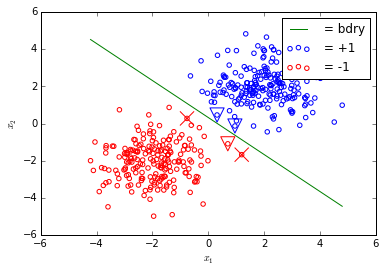
\includegraphics[scale=0.5]{svm_stdev1_train.png}
\caption{Soft-SVM solution for decision boundary of "stdev1" training dataset with $C=1$ and a linear kernel.  'X' marks support vectors that are on the margin, whereas the triangle marks support vectors that are inside the margin.}
\label{svm_stdev1}

\end{figure}
%\begin{figure}
%\centering
%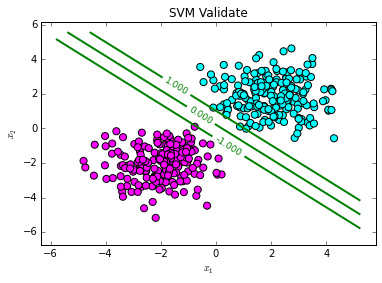
\includegraphics[scale=0.5]{svm_stdev1_val.png}
%\label{svm_toy}
%\caption{Soft-SVM solution for decision boundary of "stdev1" validation dataset with $C=1$ and a linear kernel}
%\end{figure}
\begin{figure}
\centering
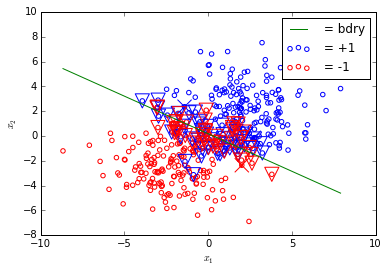
\includegraphics[scale=0.5]{svm_stdev2_train.png}
\caption{Soft-SVM solution for decision boundary of "stdev2" training dataset with $C=1$ and a linear kernel.  'X' marks support vectors that are on the margin, whereas the triangle marks support vectors that are inside the margin.}
\label{svm_stdev2}

\end{figure}
%\begin{figure}
%\centering
%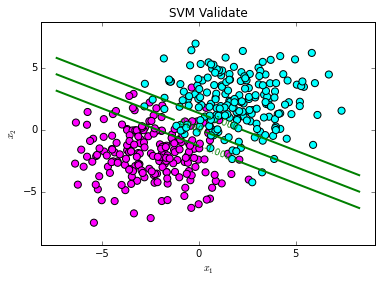
\includegraphics[scale=0.5]{svm_stdev2_val.png}
%\label{svm_toy}
%\caption{Soft-SVM solution for decision boundary of "stdev2" validation dataset with $C=1$ and a linear kernel}
%\end{figure}
%\begin{figure}
%\centering
%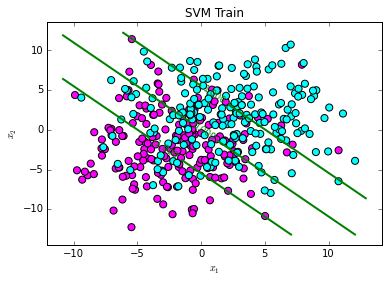
\includegraphics[scale=0.5]{svm_stdev4_train.png}
%\label{svm_toy}
%\caption{Soft-SVM solution for decision boundary of "stdev4" training dataset with $C=1$ and a linear kernel}
%\end{figure}
%\begin{figure}
%\centering
%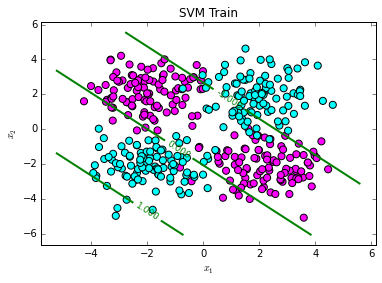
\includegraphics[scale=0.5]{svm_stdev4_val.png}
%\label{svm_toy}
%\caption{Soft-SVM solution for decision boundary of "stdev4" validation dataset with $C=1$ and a linear kernel}
%\end{figure}
%\begin{figure}
%\centering
%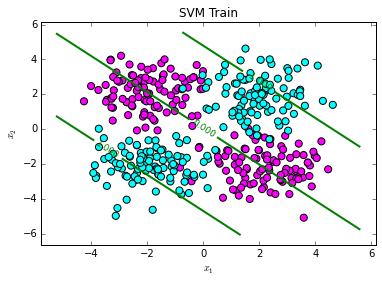
\includegraphics[scale=0.5]{svm_nonsep_train.png}
%\label{svm_toy}
%\caption{Soft-SVM solution for decision boundary of "nonsep" training dataset with $C=1$ and a linear kernel}
%\end{figure}
\begin{figure}
\centering
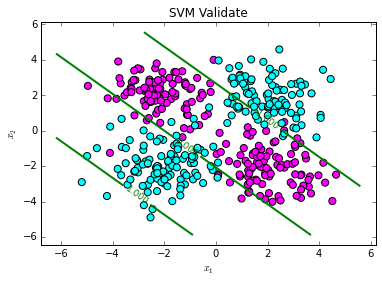
\includegraphics[scale=0.5]{svm_nonsep_val.png}
\caption{Soft-SVM solution for decision boundary of "nonsep" validation dataset with $C=1$ and a linear kernel.}
\label{svm_nonsep}
\end{figure}

The Gaussian kernel offers an interesting alternative to the linear kernel for classification.  The formulation of the SVM is exactly the same as the linear kernel except the kernel is now $k(x,x') = \exp\big( - \frac{1}{2 \sigma^2} ||x-x'||_2^2  \big)$
where $\sigma$ is termed the bandwidth.  %We can adjust both the $C$ (relative penalty on the slack variables) and bandwidth, $\sigma$, in order to tune our classifier to the data.

For both the linear kernel and the Gaussian kernel, we vary $C$ in the range $[0.0001, 500]$ and observe the effects on the classifier solution.  Increasing $C$ in general decreases $\frac{1}{||\mathbf{w}||}$, the geometric margin.  This makes sense because as $C$ is increased, the Soft-SVM formulation becomes closer to Hard-SVM, where separability of the data is required. The objective of the primal form of soft-SVM is $\frac{1}{2} ||w||^2 + C \sum_i \xi_i$. In the limit as $C \to 0$ is is clear that this objective converges to $\frac{1}{2}||w||$. Hence for very small $C$ all we care about is minimizing $||w||$ and don't care about missclassification (i.e. we don't care about the term $C \sum_i \xi_i$ since it is tending to zero). Thus $||w|| \to 0$ as $C \to 0$ which implies that $\frac{1}{||w||} \to \infty$ as $C \to 0$, as can be seen in Figures \ref{geom_lin} and \ref{geom_gauss}. 
\begin{figure}
\centering
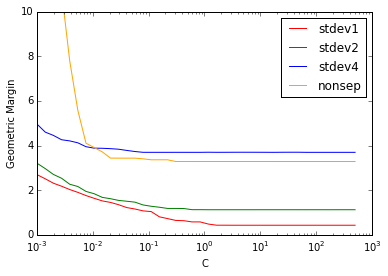
\includegraphics[scale=0.5]{geom_lin.png}
\caption{Geometric margin for 40 values of C between .001 and 500.  Computed with a linear kernel SVM.}
\label{geom_lin}
\end{figure}

\begin{figure}
\centering
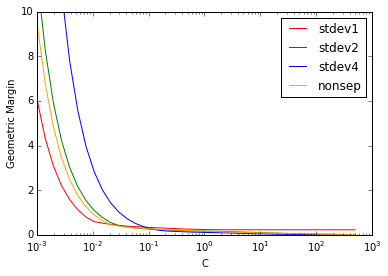
\includegraphics[scale=0.5]{geom_gauss.png}
\caption{Geometric margin for 40 values of C between .001 and 500.  Computed with a Gaussian kernel SVM, $\sigma=1$.}
\label{geom_gauss}
\end{figure}

For linearly separable data, with a linear kernel, then as $C$ is increased the number of support vectors decreases to the minimum number that is required to separate the data.  This corresponds to the weights $||\mathbf{w}||$ going to infinity as the SVM becomes increasingly ``Hard''.  An example of linearly separable data with a large ($1e9$) $C$ is provided in Figure \ref{highC}, where there are zero support vectors inside the margin.  The situation is less clean, however, for data that is not linearly separable.  This can be explained by the increasing of $C$ causing new vectors to be misclassified even if it will overall decrease the sum of the slack variables.
\begin{figure}
\centering
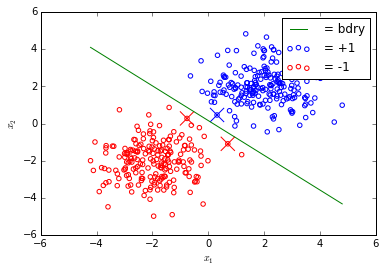
\includegraphics[scale=0.5]{svm_highC_stdev1.png}
\caption{Soft-SVM solution for decision boundary of "stdev1" training dataset with $C=1e9$ and a linear kernel.  'X' marks support vectors that are on the margin, whereas the triangle marks support vectors that are inside the margin.}
\label{highC}
\end{figure}
\begin{figure}
\centering
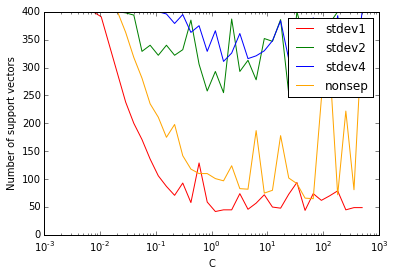
\includegraphics[scale=0.5]{supportvectors.png}
\caption{Number of support vectors as a function of $C$ for various values the range $[0.0001, 500]$ Computed with a Gaussian kernel SVM, $\sigma=1$}
\label{supportvectors}
\end{figure}

Although maximizing the geometric margin is a noble goal for an SVM classifier, it is not always the best objective function for determining the optimal $C$ to employ.  In the limit, a $C$ of $0$ will allow the SVM to misclassify as many points as needed in order to maximize the margin.  Additionally, as seen in Figure \ref{supportvectors}, small $C$ values may cause each point to become a support vector, which completely eliminates the "sparsity" advantage that SVMs may have over other classification techniques. An alternative, preferable objective for determining the optimal $C$ could be to minimize the misclassification error in cross-validation.  For consideration, the classification error rate is plotted for the validation datasets in Figure \ref{cer_svm}.
\begin{figure}
\centering
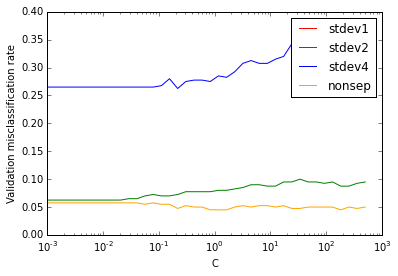
\includegraphics[scale=0.5]{cer_svm.png}

\caption{Classification error rates on the validation data sets, as a function of C for various values in the range $[0.0001, 500]$ Computed with a Gaussian kernel SVM, $\sigma=1$}
\label{cer_svm}
\end{figure}

Two additional comments on the Gaussian kernel.  First, it is nice to examine the Gaussian-kernel SVM's ability to easily classify the ``nonsep'' dataset.  With $C=\sigma=1$, for example, a misclassification error rate of $0.0475$ is achieved, which is an order of magnitude better than the linear kernel (see Figure \ref{nonsep_gaussian}).  Second, we note that for the Gaussian kernel, decreasing the bandwidth allows the classifier to perfectly overfit the training data, while increasing the bandwidth causes the decision boundary to be more smooth.  Very high bandwidth gives almost an almost linear decision boundary. The optimal bandwidth often lies somewhere in between these extremes, as can be seen in Figure \ref{bandwidth_cer}.
\begin{figure}
\centering
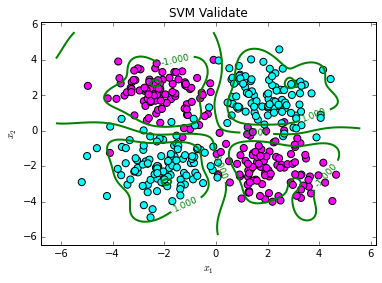
\includegraphics[scale=0.5]{nonsep_gaussian.png}
\caption{Gaussian-kernel SVM ($C=\sigma=1$) able to nicely separate the validation data for the ``nonsep'' dataset.  Classification error rate is 0.0475.}
\label{nonsep_gaussian}
\end{figure}
\begin{figure}
\centering
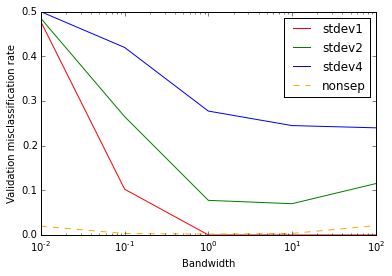
\includegraphics[scale=0.5]{bandwidth_cer.png}
\caption{Validation datasets misclassification rates for various bandwidths, $\sigma$.  Gaussian kernel and $C=1$ are used.}
\label{bandwidth_cer}
\end{figure}



\section{Titanic}

We provide below each of the required 3 questions regarding our Logistic Regression and linear-kernel SVMs on the Titanic dataset.  Before we discuss them, however, we also note for fun that we were able to achieve superior results with a Gaussian-kernel SVM: with $\sigma=10, C=100$, we achieved a misclassification rate of 0.19 on the test set and 0.12 on the validation set.

\begin{enumerate}
\item For Logistic Regression (LR), we perform ``interval'' type feature rescaling. Namely we rescale all the features so that they lie in $[0,1]$. The performance of LR is shown in Figure \ref{titanic_logit}. Performing model selection leads us to choose $\lambda = 2.5$.
 \begin{figure}
 \centering
 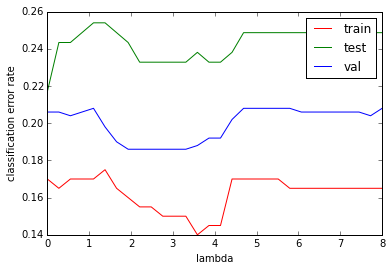
\includegraphics[scale=0.5]{titanic_logit.png}
 \caption{Results of logistic regression classifier on the Titanic dataset for different value of $\lambda$.}
  \label{titanic_logit}
 \end{figure}
 


 \item The performance of the SVM classifier is shown in Figure \ref{titanic_svm}.  Performing model selection leads us to choose $C=0.046$.  Feature scaling was also implemented, although in practice did not help as much as it did for the gradient-descent-based LR classifier.
 
   \begin{figure}
 \centering
 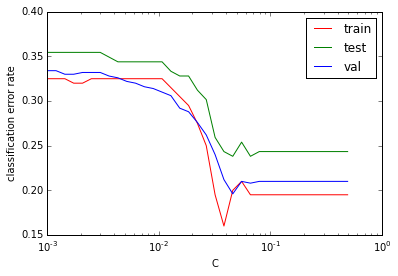
\includegraphics[scale=0.5]{titanic_svm.png}
 \caption{Results of the linear-kernel SVM classifier on the Titanic dataset for different value of $C$.}
  \label{titanic_svm}
 \end{figure}

 \item The classifiers (resulting from model selection in parts 1 and 2) for logistic regression (LR) and SVM are detailed in Table \ref{weights}. For LR we see that the most important features are which class you are in, your sex, and your age. For both LR and SVM, sex is the most important feature.  SVM has similar relative importance between weights, although age is not as important as it is for LR. Thus overall we see that logistic regression and SVM arrive at similar solutions. In particular the solutions make sense from a practical standpoint. Women were given preference to get on the lifeboats (hence the large coefficient on sex) and being in third class lowers your chances of survival. Hence both SVM and logistic regression produce sensible results for classifying the Titanic dataset.
 %
 \begin{table}[H]
 \begin{tabular}{|c|c|c|}
 \hline
 Meaning & LR & SVM \\ \hline
 $w_0$ & $-0.854$ & $-0.785$ \\ \hline
 1st Class & $0.35$ & $0.032$\\ \hline
 2nd Class & $0.33$ & $0.19$\\ \hline
 3rd Class & $-0.69$ & $-0.22$\\ \hline
 Sex  & $1.65$ & $1.27$\\ \hline
 Age & $-0.267$ & $-0.008$\\ \hline
 \# Siblings/Spouses & $-0.004$ & $-0.11$ \\ \hline
 \# Parents/Children & $0.23$ & $0.18$\\ \hline
 Fare & $0.16$ & $0.006$\\ \hline
 Southampton & $-0.255$ & $-0.08$ \\ \hline
 Cherbourg & $0.23$ & $0.12$\\ \hline
 Queenstown & $0.026$ & $-0.039$\\ \hline
 \end{tabular}
 \caption{Classification weights}
 \label{weights}
 \end{table}


\end{enumerate}

\end{document} 


% This document was modified from the file originally made available by
% Pat Langley and Andrea Danyluk for ICML-2K. This version was
% created by Lise Getoor and Tobias Scheffer, it was slightly modified  
% from the 2010 version by Thorsten Joachims & Johannes Fuernkranz, 
% slightly modified from the 2009 version by Kiri Wagstaff and 
% Sam Roweis's 2008 version, which is slightly modified from 
% Prasad Tadepalli's 2007 version which is a lightly 
% changed version of the previous year's version by Andrew Moore, 
% which was in turn edited from those of Kristian Kersting and 
% Codrina Lauth. Alex Smola contributed to the algorithmic style files.  
